\documentclass[sisc-eikonal.tex]{subfiles}

\begin{document}

\section{Ordered line integral methods for the eikonal equation}

The fast marching method discretizes the eikonal equation,
\cref{eq:eikonal}, and solves this discretization in an upwind fashion
to compute $\hat{U}$. Throughout, we distinguish between the exact
solution $u$ and the numerical solution $U$, where $\hat{U}$ will
always denote the current value to be computed. The ordered line
integral method locally and approximately minimizes the minimum action
integral of \cref{eq:eikonal}:
\begin{equation}
  \label{eq:action-functional}
  \hat{u} = \min_{\alpha} \set{u_0 + \int_\alpha s(x) dl},
\end{equation}
where $\alpha$ is a ray parametrized by arc length, $\hat{x}$ is a
target point, $\hat{u} = u(\hat{x})$, and $u_0 = u(\alpha(0))$ (see
\cref{sec:minimum-action-integral} for a derivation of
\cref{eq:action-functional}). By constrast, Lagrangian methods (i.e.,
raytracing methods) trace a bundle of rays from a common locus by
integrating \cref{eq:action-functional} for different initial
conditions. In this section, we describe our approach to discretizing
and approximately minimizing \cref{eq:action-functional}. As we
mentioned in \cref{ssec:dijkstra-like}, to compute
$\hat{U} = U(\hat{p})$ in \cref{enum:update-U} of
\cref{alg:dijkstra-like}, we need to approximately minimize several
instances of \cref{eq:action-functional}; details of this procedure
will be discussed in \cref{sec:implementation}. In this section, we
focus on a single instance of the discretized version of
\cref{eq:action-functional}, presenting our notation, deriving
prelimary results, and describing the different quadrature rules we
use, detailing useful exact solutions to the approximate minimization
of \cref{eq:action-functional}. We then present theoretical results.

\begin{figure}
  \centering
  \begin{subfigure}{.5\textwidth}
    \centering
    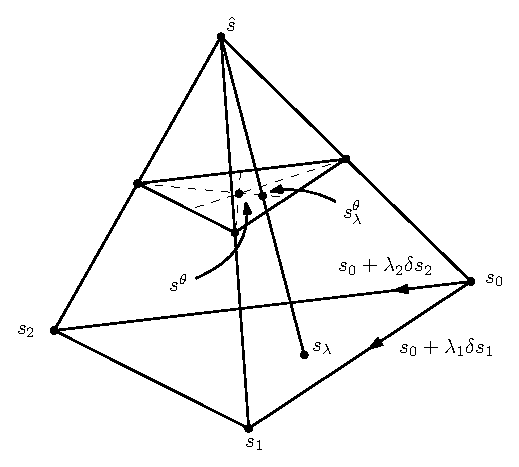
\includegraphics[width=\linewidth]{slowness-tetra.eps}
    \caption{A depiction of the different quantities related to
      $s^{\theta}$ and $s^{\theta}_\lambda$ for the case of $d = 2$, a
      tetrahedron update. Both of $s^\theta$ and $s^\theta_\lambda$ live
      on the $\theta$-section of the simplex
      $\conv(\set{\hat{p}, p_0, p_1, p_2})$. The function
      $s^\theta_\lambda$ is a linear combination of $\hat{s}, s_0, s_1$,
      and $s_2$; the value $s^\theta$ is $s^\theta_\lambda$ evaluated at
      the centroid of the $\theta$-section.}\label{fig:slowness-tetra}
  \end{subfigure}%
  \hspace{.05\linewidth}
  \begin{subfigure}{.44\textwidth}
    \centering
    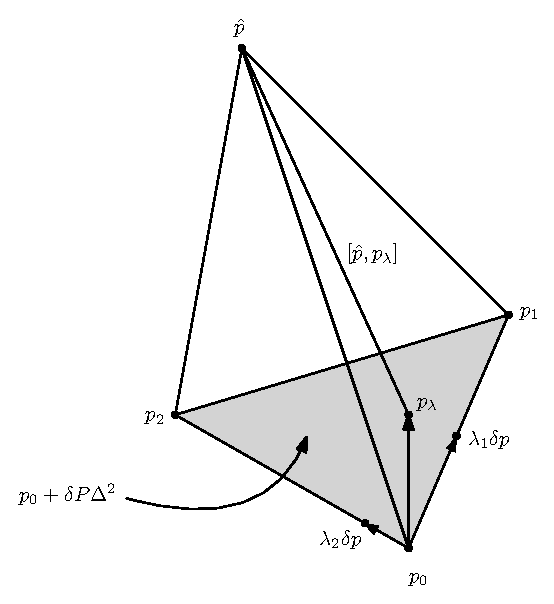
\includegraphics[width=\linewidth]{simplex-diagram.eps}
    \caption{An example showing an update interval for $d = 2$ (a
      tetrahedron update).}\label{fig:tetra-diagram}
  \end{subfigure}
  \caption{Characteristics emanate from the set
    $p_0 + \delP \Delta^d = \set{p_0 + \lambda_1 \delp_1 + \cdots +
      \lambda_d \delp_d}$, which approximates the front of the
    numerical solution. These figures depict the quantities involved
    in a tetrahedron update.}\label{fig:simplex-diagrams}
\end{figure}

\subsection{Notation}

When numerically minimizing \cref{eq:action-functional}, we minimize a
line integral whose starting point is constrained to lie on the base
of a simplex (lines, triangles, and tetrahedra in 2D and 3D). This is
depicted in \cref{fig:simplex-diagrams}. Since we solve
\cref{eq:eikonal} on a regular grid, there are only a small number of
distinct simplexes that we need to treat in our implementation, each
with fixed geometry but varying data. Because of this, it is
beneficial for us to rescale the vertices of each simplex to lie in
$\mathbb{Z}^n$ and translate each so that the point being updated lies
at the origin.

Let $n$ and $d$ be integers such that $n \geq 2$ and $0 \leq d <
n$. We think of $n$ as the ambient dimension and $d$ as the affine
dimension of the facet of the simplex where the line integral
originates (e.g., $d = 2$ for a tetrahedron). Let
$p_0, \hdots, p_d \in \Z^n \backslash \set{0}$ be linearly
independent. Together with the update point $\hat{p} = 0$, these
vectors are the vertices of a simplex with affine dimension $d$. In
this work, since we focus on the eikonal equation, we only consider
vectors $p_i$ which satisfy $\norm{p_i}_\infty = 1$ (larger
neighborhoods may be required for a Hamilton-Jacobi solver). For each
$i = 0, \hdots, d$, we also define $x_i$ to be the preimage of $p_i$
before scaling and translation is performed (i.e., $x_i$ lies in
$h \Z^n$). The numerical solution $U$ and the slowness function $s$
are evaluated at the points $x_i$; we write $U_i = U(x_i)$ and
$s_i = s(x_i)$. For a fixed update, we ``forget'' $x_i$ and think of
$U_i$ and $s_i$ being ``evaluated'' at $p_i$. For a given $n$, it is
necessary to do updates for simplexes with affine dimension up to and
including $n$. We will cover this in more detail in
\cref{sec:implementation}; presently, we will derive the updates for
general dimension since there is no need to specialize. So, for this
section, we simply assume that $d = n - 1$. Nothing important is lost
when we make this simplification.

We define the set $\Delta^d$, the parameter space for the simplex, by:
\begin{equation}\label{eq:Delta-set}
  \Delta^d = \big\{(\lambda_1, \hdots, \lambda_d) : \lambda_i \geq 0 \mbox{ for } i = 1, \hdots, d \mbox{ and } \lambda_1 + \cdots + \lambda_d \leq 1\big\}.
\end{equation}
We will also occasionally write $\Delta^d$ as a linear matrix inequality:
\begin{equation}\label{eq:Delta-LMI}
  \lambda \in \Delta^d \iff A\lambda \leq b, \hspace{1em} \mbox{where } A = \begin{bmatrix}
    -I_d \\ \m{1}_{1 \times d}
  \end{bmatrix} \in \mathbb{R}^{d + 1 \times d}, \hspace{1em} \mbox{and }
  b = \begin{bmatrix} \m{0}_{d \times 1} \\ 1 \end{bmatrix} \in \mathbb{R}^{d + 1}.
\end{equation}
For each $\lambda = (\lambda_1, \hdots, \lambda_d) \in \Delta^d$, we
will write $\lambda_0 = 1 - \lambda_1 - \cdots - \lambda_d$. Then,
$\sum_{i=0}^d \lambda_i p_i$ lies in the convex hull of
$\set{p_0, \hdots, p_d}$. We denote this vector by $p_\lambda$ (see
\cref{fig:simplex-diagrams}). Defining $\delp_i = p_i - p_0$, we
can also write $p_\lambda = p_0 + \sum_{i=1}^d \lambda_i \delp_i$
and define the matrix:
\begin{equation}
  \delP = \begin{bmatrix} \delp_1 & \cdots & \delp_d \end{bmatrix} \in \R^{n \times d},
\end{equation}
so that we can write $p_\lambda = \delP \lambda + p_0$. Along the
same lines, $U_\lambda = U_0 + \delU^\top \lambda$, where
$\delU_i = U_i - U_0$; we also define
$s_\lambda = s_0 + \dels^\top \lambda$, where
$\dels_i = s_i - s_0$. Although the slowness function $s$ may be
available to us in analytic form, we assume that it is only available
on the nodes in $\calG$ to reflect use in real-world applications
(e.g., $s$ will most likely be presented to use on a grid as some
form.

\subsection{Quadrature}\label{ssec:quadrature}

To minimize \cref{eq:action-functional}, we assume that $\alpha$ is a
line segment parametrized by arc length and then apply several
different one-point quadrature rules to the resulting integral. If
$\alpha$ is a line segment connecting $p_\lambda$ and $\hat{p} = 0$,
then:
\begin{equation}
  \label{eq:action-functional-line-segment}
  \hat{U} = U(\hat{p}) = \min_{\lambda \in \Delta^d} \set{U_\lambda + h \int_{[p_\lambda, 0]} s(\alpha(t))dt}.
\end{equation}
We consider two approximations to
\cref{eq:action-functional-line-segment}. Let
$l_\lambda = \norm{p_\lambda}_2$. For $\theta$ such that
$0 \leq \theta \leq 1$, we define:
\begin{align}
  F_0(\lambda) = F_0^\theta(\lambda) &= U_\lambda + s^{\theta} h l_\lambda := U_\lambda + \squareb{(1-\theta)\hat{s} + \frac{\theta}{d + 1} \sum_{i=0}^d s_i} h l_\lambda, \label{eq:f0-definition} \\
  F_1(\lambda) = F_1^\theta(\lambda) &= U_\lambda + s^{\theta}_\lambda h l_\lambda := U_\lambda + \squareb{(1-\theta)\hat{s} + \theta s_\lambda} h l_\lambda,
\end{align}
where we omit the superscript in $F_i^\theta$ when the context is
clear. We primarily concern ourselves with $F_0$ and $F_1$ where
$\theta = 0$ and $\theta = \nicefrac{1}{2}$. See
\cref{fig:slowness-tetra} for a careful explanation of this setup. If
$\theta = 0$, then $F_0 \equiv F_1$, so we define a single quadrature
rule to capture this case, which we call \texttt{rhr}. If
$\theta = \nicefrac{1}{2}$, then $F_0 \neq F_1$ in general, leading us
to define a separate midpoint quadrature rule for each of $F_0$ and
$F_1$, named \texttt{mp0} and \texttt{mp1}, respectively. The case of
\texttt{mp0} requires special care and is handled in
\cref{ssec:validation}. The distinction between these quadrature rules
and their impact on our solvers is a key consideration of this paper.

\subsection{The minimization problem}\label{ssec:minimization-problem}

With $F_0$ and $F_1$ so defined, the minimization problem which
approximately solves \cref{eq:action-functional-line-segment} to
compute $\hat{U}$ for a fixed update simplex is:
\begin{equation}
  \label{eq:constrained-minimization}
  \hat{U} = \min_{\lambda \in \Delta^d} F_i(\lambda).
\end{equation}
This is a nonlinear, constrained optimization problem with linear
inequality constraints and no equality constraints (cf.\@
\cref{eq:Delta-LMI}). We require the gradient and Hessian of $F_0$ and
$F_1$ for our algorithms and analysis. These are easy to compute, but
we have found a particular form for them to be convenient. The proofs
of these propositions and the rest of the results in
\cref{ssec:minimization-problem} are found in
\cref{sec:minimization-proofs}.

\begin{proposition}\label{prop:F0-grad-and-Hess}
  The gradient and Hessian of $F_0(\lambda; \theta)$ satisfy:
  \begin{align}
    \nabla F_0(\lambda) &= \delU + s^{\theta} h \delP^\top \nu_\lambda,\label{eq:F0-grad} \\
    \nabla^2 F_0(\lambda) &= \frac{s^{\theta} h}{l_\lambda} \delP^\top \calP^\perp_{p_\lambda} \delP,
  \end{align}
  where $\nu_\lambda = p_\lambda/l_\lambda$ is the unit vector in the
  direction of $p_\lambda$,
  $\calP_{p_\lambda} = \nu_\lambda \nu_\lambda^\top$ denotes the
  orthogonal projector onto $\operatorname{span}(p_\lambda)$ and
  $\calP_{p_\lambda}^\perp = I - \nu_\lambda \nu_\lambda^\top$ is the
  orthogonal projector onto $\operatorname{span}(p_\lambda)^\perp$,
  the orthogonal complement of $\operatorname{span}(p_\lambda)$.
\end{proposition}

\begin{proposition}\label{prop:F1-grad-and-Hess}
  The gradient and Hessian of $F_1(\lambda; \theta)$ satisfy:
  \begin{align}
    \nabla F_1(\lambda) &= \delU + \theta h l_\lambda \dels + s^{\theta}_\lambda h \delP^\top \nu_\lambda, \\
    \nabla^2 F_1(\lambda) &= \set{\delP^\top \nu_\lambda, \theta h \dels} + \frac{s^\theta_\lambda h}{l_\lambda} \delP^\top \calP^\perp_{p_\lambda} \delP, \label{eq:hess-F1}
  \end{align}
  where $\set{a, b} = ab^\top + ba^\top$ is the anticommutator of two
  vectors.
\end{proposition}

Our task is to minimize $F_0$ and $F_1$ over the convex set
$\Delta^n$; so, we need to determine whether $F_0$ and $F_1$ are
convex themselves. The next two lemmas address this point. We also
examine whether $F_0$ and $F_1$ are strictly convex or just
convex. This relates to the definiteness of their Hessians, computed
above.

\begin{lemma}\label{lemma:dPt-cprojp-dP-pd}
  Let $p_0, \hdots, p_d$ form a nondegenerate simplex (i.e.,
  $p_0, \hdots, p_d$ are linearly independent) together with $\hat{p}$
  and assume that $s$ is positive. Then, $\nabla^2 F_0$ is positive
  definite and $F_0$ is strictly convex.
\end{lemma}

For $F_1$, we can only obtain convexity (let alone strict convexity)
for $h$ sufficiently small. For large enough $h$, we will encounter
nonconvex updates. To obtain convexity, we need to stipulate that the
slowness function $s$ be Lipschitz continuous on $\Omega$ with a
Lipschitz constant that is constant independent of $h$. In practice,
we have not found this to be a particularly stringent restriction.

\begin{lemma}\label{lemma:F-strictly-convex}
  Again, assume that the update simplex is nondegenerate and that $s$
  is positive. Additionally, assume that $s$ is Lipschitz continuous
  with Lipschitz constant $K \leq C$ on $\Omega$, for some constant
  $C > 0$ independent of $h$. Then, $\nabla^2 F_1$ is positive
  definite (hence, $F_1$ is strictly convex) for $h$ small enough.
\end{lemma}

We have found that all \texttt{mp1} updates become strictly convex
problems rapidly as $h \to 0$. The reason for this is discussed at the
end of \cref{ssec:causality}.

\subsection{Validation of \texttt{mp0}}\label{ssec:validation}

If we consider an update simplex defined by the nodes
$p_0, \hdots, p_{n-1}$, each subset of these nodes defines another,
lower-dimensional update simplex, which lies on the boundary of the
original simplex. For example, three triangle updates form the
boundary of a single tetrahedron update. We expect the values of $F_i$
to be the same whether defined on one or another incident update
simplex, and to be continuous as we transfer between simplexes that
share a common boundary. For $F_1$ this is the case, but for $F_0$
with $\theta \neq 0$, the function $F_0$ may not be well-defined or
continuous at boundaries. This problem can lead to inconsistent and
divergent solvers. A heuristic fix is to first minimize
\cref{eq:constrained-minimization} for $F_0$ with nonzero $\theta$ to
obtain the minimizing argument $\lambda^*_0$, then set
$\hat{U} = F_1(\lambda_0^*)$; i.e., to replace $F_0$ with $F_1$ for
the purposes of evaluation, or to use $F_0$ as a surrogate when
minimizing $F_1$.

If we use Newton's method to minimize $F_1$, starting from
$\lambda_0^*$ and letting $\lambda_1^*$ denote the optimum of
\cref{eq:constrained-minimization} for $F_1$, then we can use use the
convergence theory of Newton's method to prove the following result
which bounds the distance between $\lambda_0^*$ and $\lambda_1^*$,
thereby bounding the error incurred by using \texttt{mp0} instead of
\texttt{mp1}~\cite{stoer2013introduction}.

\begin{theorem}\label{theorem:mp0-newton}
  Let $h$ be sufficiently small so that $F_1$ is strictly convex (see
  \cref{lemma:F-strictly-convex}). Then, the error
  $\dellam^* = \lambda_1^* - \lambda_0^*$ satisfies
  $\norm{\dellam^*} = O(h)$. Further, if we let
  $\lambda_0 = \lambda_0^*$ in the following Newton iteration:
  \begin{equation}
    \label{eq:lam0-iter-to-lam1}
    \lambda_{k+1} \gets \lambda_k - \nabla^2 F_1(\lambda_k)^{-1} \nabla F_1(\lambda_k), \qquad k = 0, 1, \hdots,
  \end{equation}
  then this iteration is well-defined, and converges quadratically to
  $\lambda_1^*$. This immediately implies that the error incurred by
  \texttt{mp0} is $O(h^3)$ per update compared to \texttt{mp1}; i.e.:
  \begin{equation}
    \label{eq:mp0-error}
    \abs{F_1(\lambda_1^*) - F_1(\lambda_0^*)} = O(h^3).
  \end{equation}
\end{theorem}

\begin{proof}
  The proof of \cref{theorem:mp0-newton} is detailed in
  \cref{app:validation-proofs}.
\end{proof}

We can provide some intuition for why this bound is satisfactory. If
we assume that our domain is spanned along a diameter by $O(N)$ nodes,
and that $h \sim N^{-1}$, then we can anticipate $O(N)$ downwind
updates, starting from $\boundary$ and extending to the boundary of
$\calG$ in any direction. Accumulating the error over these nodes, we
can expect the maximum pointwise error between a solution to
\cref{eq:eikonal} computed by using \texttt{mp0} and \texttt{mp1} to
be $O(h^2)$, which is dominated by the $O(h)$ discretization error
coming from the linear convergence of the method itself.

If we exchange the roles of $F_0$ and $F_1$ (if we start from
$\lambda_1^*$ and perform a Newton iteration on $\nabla F_0$) we can
obtain the foregoing error bound again. The main reason to start from
$\lambda_0^*$ and iterate to $\lambda_1^*$ is that it allows us to use
\texttt{mp0} to initialize \texttt{mp1}. Indeed, in the next section,
we will see that it is possible to perform \texttt{mp0} updates
without resorting to a nonlinear solver, but that this is not the case
for \texttt{mp1}. For $d = 0$, this is unimportant, but for
$d \geq 1$, minimizing $F_0$ can be cheaper. Reducing the number of
$F_1$ update iterations leads to a sped-up method with the same
accuracy.

\subsection{Exact solution for \texttt{rhr} and \texttt{mp0}}\label{ssec:exact-soln}

Since $F_0$ is strictly convex, $\nabla F_0(\lambda) = 0$ is
sufficient for the optimality of $\lambda$. The system of nonlinear
equations defined by $\nabla F_0(\lambda) = 0$ can be solved exactly
without an iterative solver. We can compute the solution using the
reduced QR decomposition of $\delP$ and after some geometric
consideration of the minimization problem. This is captured by the
following theorem, with the geometry of the problem is depicted in
\cref{fig:f0-exact}.

\begin{theorem}\label{thm:f0-exact}
  Let $\delP = QR$ be the reduced QR decomposition of $\delP$; i.e.,
  where
  $Q \in \mathbb{R}^{n \times d}, R \in \mathbb{R}^{d \times d},
  Q^\top Q = I_d$, and with $R$ upper triangular. For $s^\theta, h$,
  and $U$ fixed, if
  $\lambda^* = \argmin_{\lambda \in \mathbb{R}^n}
  F_0^\theta(\lambda)$, then:
  \begin{align}
    l_{\lambda^*} &= \sqrt{\frac{p_0^\top {(I - QQ^\top)} p_0}{1 - \norm{R^{-\top} \frac{\delU}{s^\theta h}}^2}},\label{eq:l-star-expression} \\
    \lambda^* &= -R^{-1} \parens{Q^\top p_0 + l_{\lambda^*} R^{-\top} \frac{\delU}{s^\theta h}},\label{eq:f0-exact-lambda} \\ 
    \hat{U} &= U_0 + \frac{s^\theta h}{l_{\lambda^*}} p_0^\top p_{\lambda^*}.\label{eq:f0-exact}
  \end{align}
\end{theorem}

\begin{proof}
  See \cref{sec:exact-soln-proofs}.
\end{proof}

\subsection{Equivalence of the upwind finite difference scheme and
  $F_0$}\label{ssec:equivalence}

If we linearly approximate $U$ near $\hat{p}$, then for
$i = 0, \hdots, n - 1$, we find that $\hat{U}$ approximately
satisfies:
\begin{equation}
  \label{eq:finite-differences}
  U_i - \hat{U} = \nabla \hat{U}^\top p_i.
\end{equation}
This finite difference approximation to \cref{eq:eikonal} can be
solved exactly and is a known generalization of the upwind finite
difference scheme used by the fast marching method to an unstructured
mesh~\cite{kimmel1998computing,sethian2000fast}. Computing $\hat{U}$
using this approximation is equivalent to solving:
\begin{equation}
  \hat{U} = \min_{\lambda \in \Delta^n} F_0(\lambda)
\end{equation}
in a sense made precise by the following theorem.

\begin{theorem}[Equivalence of upwind finite difference scheme and $F_0$]\label{thm:equivalence}
  Let $\hat{U}$ by the solution of \cref{eq:finite-differences} and
  let $\hat{U}' = \min_{\lambda \in \R^n} F_0(\lambda)$. Then,
  $\hat{U}$ exists if and only if
  $\|R^{-\top} \delU\| \leq s^\theta h$, and can be computed from:
  \begin{equation}
    \label{eq:U-finite-diff}
    \hat{U} = U_i - p_i^\top Q R^{-\top} \delU + \norm{\pmin} \sqrt{{(s^\theta h)}^2 - \norm{R^{-\top} \delU}^2},
  \end{equation}
  where $\pmin = (I - QQ^\top) p_i$ (for any $i$, see
  \cref{fig:f0-exact} in \cref{sec:exact-soln-proofs}). Additionally,
  the following hold:
  \begin{enumerate}
  \item The finite difference solution and line integral solution
    coincide: i.e., $\hat{U} = \hat{U}'$ can be computed from:
    \begin{equation}
      \label{eq:U-from-Ui-exact}
      \hat{U} = U_i + s^\theta h p_i^\top \nu_{\lambda^*},
    \end{equation}
    where $\lambda^* = \argmin_{\lambda \in \R^n} F_0(\lambda)$ and
    $\nu_{\lambda^*} = p_{\lambda^*}/l_{\lambda^*}$.
  \item The characteristics found by solving the finite difference
    problem and minimizing $F_i$ coincide and are given by
    $[p_{\lambda^*}, \hat{p}] = [p_{\lambda^*}, 0]$.
  \item The approximated characteristic passes through
    $\conv(\set{p_0, \hdots, p_{n-1}})$ if and only if
    $\lambda^* \in \Delta^n$.
  \end{enumerate}
\end{theorem}

\begin{proof}
  See \cref{sec:equivalence-proofs}.
\end{proof}

\subsection{Causality}\label{ssec:causality} Dijkstra-like
methods are based on the idea of monotone causality, similar to
Dijkstra's method itself. To compute shortest paths in a network,
Dijkstra's method uses dynamic programming to compute globally optimal
shortest paths using local information~\cite{dijkstra1959note}. In
this way, the distance to each downwind vertex must be greater than
its upwind neighboring vertices. In the continuous setting, for our
scheme to converge to the correct viscosity solution, it is necessary
for our scheme to be consistent and
monotone~\cite{crandall1983viscosity}. Our methods based on the
\texttt{rhr} and \texttt{mp0} quadrature rules automatically inherit
the consistency and causality of the finite difference methods that
they relate to if they use the same 4 or 6 point neighborhoods in 2D
and 3D. We consider many different update neighborhoods involving
geometrically distinct simplexes. To this end, we provide a simple way
of checking whether each simplex is causal.

The causality of an update depends on the underlying simplex and the
problem data. In particular, an update is causal for $F_i$ if:
\begin{equation}
  \hat{U} = F_i(\lambda_i^*) \geq \max_i U_i.
\end{equation}
It is enough to determine whether or not each type of update simplex
admits only causal updates, which relates to whether the simplex is
acute.

We also consider something we refer to here as the ``update gap'': the
difference $\hat{U} - \max_i U_i$. As discussed in Tsitsiklis's
original paper~\cite{tsitsiklis1995efficient}, an alternative to
Dijkstra's algorithm is Dial's algorithm---a bucketed version of
Dijkstra's algorithm which runs in $O(N)$ time, where the constant
depends on the bucket size~\cite{dial1969algorithm,kim2001calo}. In
this case, the size of the buckets is determined by the update gap. It
is unclear whether there is any real advantage of a Dial-like solver
(see~\cite{jeong2008fast} for a discussion). We present numerical
evidence suggesting that this is not the case in (\textbf{TODO}: cite
subsection). Despite this, the update gap is of fundamental importance
and limits the number of nodes that can be processed in parallel
without breaking causality.

We now present a simple characterization of causality and a way to
compute the update gap.
\begin{theorem}\label{thm:causality}
  An update simplex is causal for $F_0$ if and only if
  $\nu_i^\top \nu_j \geq 0$ for all $i$ and $j$ such that
  $0 \leq i < n$ and $0 \leq j < n$. If we assume that $s$ is
  Lipschitz continuous, for $h$ small enough, the simplex is also
  causal for $F_1$, and the term in $F_1$ which prevents an update
  from being causal decays with order $O(h^2)$. Furthermore, the
  update gap is given explicitly by:
  \begin{equation}
    \hat{U} - \max_i U_i = s^\theta h \min_{i, j} \frac{\nu_i^\top \nu_j}{\norm{p_i}}.
  \end{equation}
\end{theorem}

\begin{proof}
  See \cref{sec:equivalence-proofs}.
\end{proof}

\noindent The fact that the term in $F_1$ which can prevent causality
for large $h$ is $O(h^2)$ accounts for the phenomenon that for all
practical problem sizes the method is causal and converges.

\end{document}

%%% Local Variables:
%%% mode: latex
%%% TeX-master: "sisc-eikonal.tex"
%%% End:
